\documentclass[10pt,a4paper]{article}
\usepackage[utf8]{inputenc}
\usepackage[german]{babel}
\usepackage[T1]{fontenc}
\usepackage{amsmath}
\usepackage{amsfonts}
\usepackage{amssymb}
\usepackage{graphicx}
\author{Erik Zimmermann}
\begin{document}
\section{Aggregatzustände}
\begin{itemize}
\item (fest, flüssig, gasförmig)
\item Aggregatzustände sind u.a. von Druck und Temperatur abhängig:
\end{itemize}
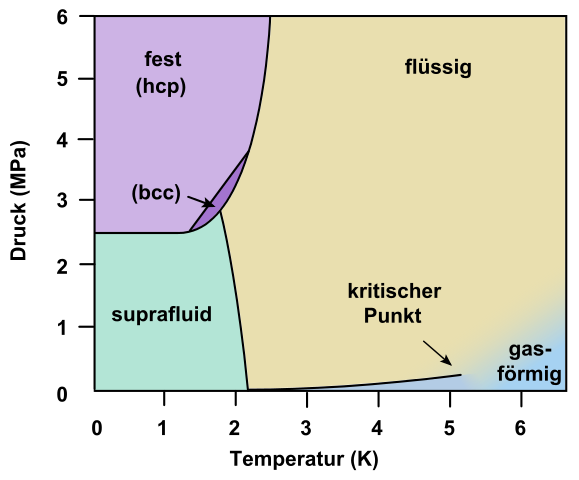
\includegraphics[scale=0.4]{579px-He4_de.png} \\\\
folgende Übergänge sind möglich:
\begin{itemize}
\item    Schmelzen (Übergang von fest zu flüssig)
\item    Verdampfen (Übergang von flüssig zu gasförmig)
\item    Sublimieren (Übergang von fest zu gasförmig)
\item    Erstarren/ Gefrieren (Übergang von flüssig zu fest)
\item    Kondensieren (Übergang von gasförmig zu flüssig)
\item    Resublimieren (Übergang von gasförmig zu fest)
\end{itemize}
\newpage
\section{kritischer Punkt}
In der Thermodynamik ist der kritische Punkt ein thermodynamischer Zustand eines Stoffes, der sich durch Angleichen der Dichten von flüssiger und Gasphase kennzeichnet. Die Unterschiede zwischen beiden Aggregatzuständen hören an diesem Punkt auf zu existieren. Im Phasendiagramm stellt der Punkt das obere Ende der Dampfdruckkurve dar:
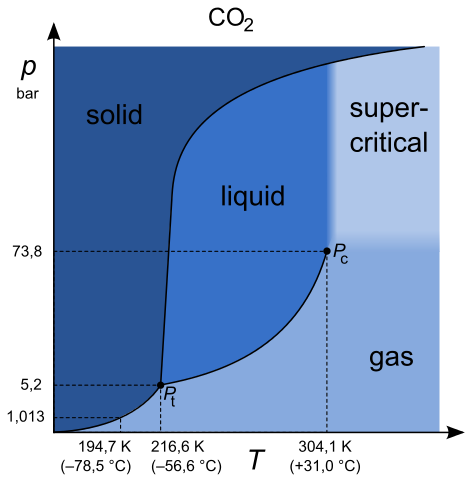
\includegraphics[scale=0.5]{472px-Carbon_dioxide_p-T_phase_diagram.png}\newpage
\section{Tripelpunkt}
In der Thermodynamik ist der Tripelpunkt (auch Dreiphasenpunkt) der Zustand, beschrieben durch Druck und Temperatur, an dem drei Aggregatzustände eines Stoffes im thermodynamischen Gleichgewicht sind.
Der Tripelpunkt ist im Phasendiagramm der Schnittpunkt der beiden Phasengrenzlinien Sättigungsdampfdruck und Schmelzkurve:
\begin{figure}[hbtp]
\centering
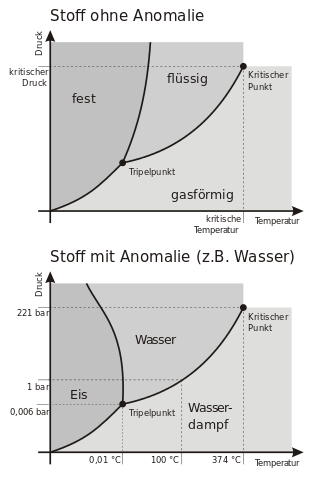
\includegraphics[scale=0.6]{316px-Phasendiagramme.png}
\end{figure} \\
(Anomalie: (gr.: Unebenheit) wie z.B. beim Wasser: niedrigster Druck bei $4 C$ und nicht $0 C$)
\end{document}
